% !TeX root = ../diss.tex

% sketch out what plots to include here
% - plot of kl divergence w.r.t. number of samples taken
% - plot of running time w.r.t. amount of data conditioned on
% - plot of running time w.r.t. number of particles (for smc)
% - maximum memory footprint (against parameters as above)
% - total memory footprint over time
% box plots instead of just lines

% use ppl to do evaluation? good to show code in my language which does evaluation

% explain WHY in evaluation, how just what - e.g. explain why plot looks how it does, don't just describe

% show some output from merlin to show the fact that type inference works and is good?
So far, I have developed a PPL that can be used to define arbitrary probabilistic models and perform Bayesian inference on them. To evaluate the performance of my PPL, I will present some examples to show programs written in my PPL translated into equivalent programs in other PPLs, and then measure time and memory consumption of inference\footnote{All tests are carried out on a single core of an Intel\textsuperscript{(R)} Core\textsuperscript{(TM)} i5-7200U CPU @ 2.50GHz}. I will also determine the correctness of inference procedures by using hypothesis tests which use drawn samples to determine whether two distributions are the same or not.

\section{Examples}
To show how my PPL would be used on real problems, I now outline a set of example problems. Several examples here will be simple, and have analytic solutions - this is so that I can then test the correctness of applying inference on them. More complex realistic models are also included to test performance. Full derivations of the solutions as well as mathematical descriptions of the models are given in appendix \ref{app:examples}.

\subsection{Sprinkler}
% to show exact inference on discrete model
The sprinkler model is a commonly used example in Bayesian inference due to it's simplicity. It is an example of a \textit{Bayesian network}, and can be visualised as in figure \ref{fig:sprinkler-network}. The code in listing \ref{lst:sprinkler} shows the model in the diagram encoded as a program. This particular program can be used (by applying an inference function) to find the probability of rain given that the grass is wet.

% \begin{noindent}
\begin{figure*}[!htb]
	\centering
	\begin{minipage}{0.47\linewidth}
		\ocamlcode{code_snippets/sprinkler.ml}	
		\captionof{listing}{Sprinkler model in code}
		\label{lst:sprinkler}						
	\end{minipage}
	\begin{minipage}{0.47\linewidth}
		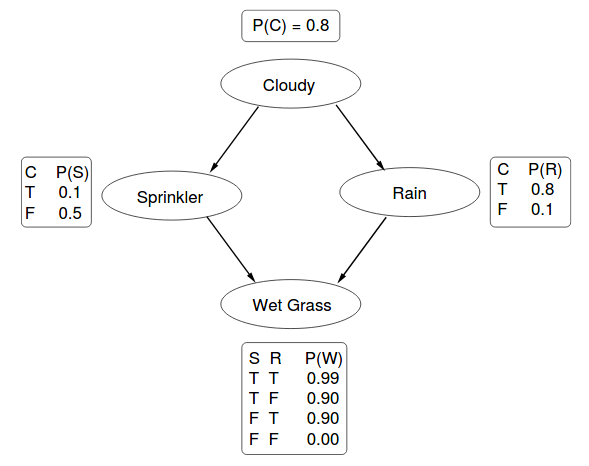
\includegraphics[width=\linewidth]{figs/sprinkler-network.png}
		\captionof{figure}{Sprinkler model as a network}
		\label{fig:sprinkler-network}
		\vspace{0.3cm}
		\begin{ocamlcode-in}
let () =
  exact_inference sprinkler_model
  |> print_exact_bool
(*false: 0.13706 true: 0.86294*)
		\end{ocamlcode-in}
		\captionof{listing}{Output of inference}
		\label{lst:inf-output}					
	\end{minipage}
	\begin{minipage}{0.47\linewidth}
	\end{minipage}
	
	% \caption{}
	% \label{}
\end{figure*}
% \end{noindent}

% \begin{listing}[!ht]
% 	\ocamlcode{code_snippets/sprinkler.ml}	
% 	\caption{Sprinkler model}
% 	\label{lst:sprinkler}
% \end{listing}

% \begin{figure}[!htb]
% 	\centering
% 	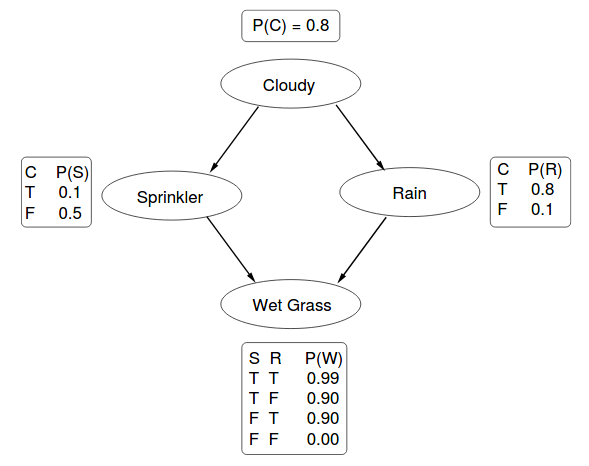
\includegraphics[width=0.5\textwidth]{figs/sprinkler-network.png}
% 	\caption{Bayesian Network example}
% 	\label{fig:sprinkler-network}
% \end{figure}

\subsection{Biased Coin} \label{sec:coin} 
% to show analytically solvable continuous distribution
% include graph of beta compared to computed posterior
Modelling a biased coin shows an example of a very simple model with a continuous posterior that can be calculated analytically \cite{datasci}. 
% 
The model is of a coin that is tossed $n$ times to give $x$ heads. We do not know if the coin is biased or not, and would like to find out the bias, $p$ of the coin, where $p$ is the probability of heads, with $p=0.5$ being an unbiased coin.
% 
To find the posterior, we use an uninformative prior ($\Theta$), the uniform. This results in the posterior, the beta distribution, specifically Beta$(x+1,n-x+1)$.

The program in my PPL is shown in listing \ref{lst:coin}, and demonstrates setting up the model, performing inference as well as finding the mean of the posterior. The application is to find the chance of the next coin flip landing heads. This example uses $n=10$ and $x=9$, so the mean produced is roughly 0.83, the mean of Beta$(10,2)$.

\begin{listing}[!ht]
	\ocamlcode{code_snippets/coin.ml}	
	\caption{Coin model}
	\label{lst:coin}
\end{listing}


\begin{figure}[!htb]
	\begin{minipage}{0.5\textwidth}
		\centering
		\jscode{code_snippets/webppl/coin.js}
		\captionof{listing}{WebPPL}
	\end{minipage}
	\begin{minipage}{0.5\textwidth}
		\centering
		\clojurecode{code_snippets/anglican/coin.clj}
		\captionof{listing}{Anglican}
	\end{minipage}
	\caption{The coin model in WebPPL (JS) and Anglican (Clojure)}
	\label{fig:compare-coin}
\end{figure}

The comparison given in Figure \ref{fig:compare-coin} shows how the same model is defined in other languages. Both languages use similar constructs, despite differing syntax. This example also shows that my PPL is similar to existing systems, and is not more verbose.

\subsection{HMM}
Hidden Markov models are slightly more involved models, where we have a sequence of hidden states, which emit observed states. There are two distributions involved here, the transition distribution, which defines how likely the next state is given the current state, and the emission distribution, which is the distribution over the observed states given the hidden state. The example in Listing \ref{lst:hmm} uses discrete distributions, but any type of distribution can be used. The exact posterior for simple models can be found using the forward-backward algorithm.
% use forward-backward to get exact posterior
\begin{listing}[!ht]
	\ocamlcode{code_snippets/hmm.ml}
	\caption{Hidden Markov Model}
	\label{lst:hmm}
\end{listing}

\subsection{Linear Regression}
This example shows how to use multiple data points to infer a continuous distribution. This example can be used to infer the parameters of a line through a set of 2-D points. The fold function can be used to condition on many observations easily. The fmap function is used to map outputs from a distribution. Since the linreg model produces tuples of parameters, we can create individual distributions over either one.

\begin{listing}[!ht]
	\ocamlcode{code_snippets/linreg.ml}	
	\caption{Linear Regression}
	\label{lst:linreg}
\end{listing}

\subsection{Infinite Mixture Model}
This example demonstrates a model which cannot be expressed in some PPLs such as STAN or Infer.Net, since it is a non-parametric Bayesian model. This is a Dirichlet Process mixture model with an infinite number of Gaussians\cite{dpmm}. It is used for the common task of clustering a set of data points without knowledge of the number of clusters. This means the number of clusters is allowed to grow with the dataset size. We use a mixture of Gaussians, meaning the likelihood of a point belonging to each cluster is given by different normal distributions. The full code for this model, along with comparisons to other languages is given in appendix \ref{app:dp}.
% Need to show examples which can't be done in graph based thing
% Need to explain why these examples are actually difficult.
% http://www.cs.cmu.edu/~epxing/Class/10708-16/slide/lecture18-DP.pdf
% This is a non-parametric Bayesian model - 
% no. of params is infinite, grows with size of dataset


\section{Statistical tests}
To evaluate the correctness of my PPL, I used statistical tests which measure goodness-of-fit, i.e. how similar two distributions are to each other. I compare the empirical distribution of 10,000 samples from an approximated distribution to an exact distribution which is calculated analytically. Test statistic distributions (e.g. the $\chi^2$ distribution) were calculated using \texttt{Owl}, and empirical distributions generated using the \texttt{EmpiricalDist} modules.

For all tests described below, I set the significance level, $\alpha = 0.05$ and use null and alternative hypotheses as follows:

$H_0:$ The sample data follow the exact distribution\\
$H_1:$ The sample data do not follow the exact distribution

\subsection{Chi-squared}

The $\chi^2$ test is a simple goodness-of-fit test which can test whether or not a given discrete distribution. The test statistic is as follows, with each $i$ being a distinct element in the distribution, $x_i$ is the observed number of samples with the value $i$, and $m_i$ is the expected number of samples for the value $i$.

$$X^{2}=\sum _{i=1}^{k}{\frac {(x_{i}-m_{i})^{2}}{m_{i}}}$$

This test statistic is compared against the critical value (at the significance level) of the chi-squared distribution, with the degrees of freedom being $k-1$, where k is the number of possible values of the distribution.
\subsubsection{Results}
\begin{table}[!ht]
	\centering
	\csvautotabular{data/hypothesis-chi.csv}
	\caption{p-values of $\chi^2$ test on different models using different inference procedures}
	\label{tab:chi-pvals}
\end{table}

Table \ref{tab:chi-pvals} shows the results of carrying out the test on several inference procedures for different discrete models. None of the values are below 0.05, so we cannot reject the null hypothesis, so we conclude that, at the 5\% significance level, the distributions are not significantly different.

\subsection{Kolmogorov-Smirnov}

The Kolmogorov-Smirnov test is a non parametric test which is used to compare a set of samples with a distribution - this is the one-sample K-S test. There is also a two-sample K-S test, which compares two sets of samples against each other. I use the one-sample test here to compare samples taken from the inferred posteriors to their exact analytic solutions.

The test statistic is as follows, with $F_n(x)$ being the empirical cumulative distribution of n samples, and $F(x)$ being the exact cumulative distribution.
\begin{align*}
	F_{n}(x) & =\frac{1}{n}\sum_{i=1}^{n}I_{[-\infty ,x]}(X_{i}) \\
	D_{n}    & =\sup_{x}|F_{n}(x)-F(x)|                          
\end{align*}
This test statistic is compared against the critical values of the Kolmogorov distribution, rejecting the null hypothesis if $\sqrt{n}D_n > K_\alpha$, where $K_\alpha$ is the critical value at the significance level $\alpha$, and $n$ is the number of samples.

\subsubsection{Results}

Table \ref{tab:ks-pvals} shows that for all the continuous models considered, the p-value obtained from all tests are greater than then 0.05. This means we do not reject $H_0$ for any model/inference procedure combination, so can be confident (at the 5\% significance level) that the inference procedures are correct. This shows that the generated posterior is not significantly different from the real solution.

\begin{table}[!ht]
	\centering
	% \begin{tabular}{|l|l|l|l|l|}
	% 	\hline
	% 	            & rejection & importance & metropolis-hastings & particle filter \\ \hline
	% 	single coin &           &            &                     &                 \\ \hline
	% 	hmm         &           &            &                     &                 \\ \hline
	% \end{tabular}
	\csvautotabular{data/hypothesis-ks.csv}
	\caption{p-values of K-S test on different models using different inference procedures}
	\label{tab:ks-pvals}
\end{table}


\section{Convergence of sampling}
% TODO: add a few lines to show difference between 
I also used the KL-divergence metric to determine the (dis)similarity of two distributions. The formula for KL Divergence of discrete distributions $P$ and $Q$ is easy to calculate by \eqref{eq:kl_disc}

$${D_{\text{KL}}(P\parallel Q)=\sum _{x\in {\mathcal {X}}}P(x)\log \left({\frac {P(x)}{Q(x)}}\right)}$$ \label{eq:kl_disc}

The continuous version is similar, with $p$ and $q$ now being density functions as in \eqref{eq:kl_cont}. 

$${D_\text{KL}}(P\parallel Q)=\int _{-\infty }^{\infty }p(x)\log \left({\frac {p(x)}{q(x)}}\right)\,dx$$ \label{eq:kl_cont}

% Since we cannot compute this integral exactly (we only have the exact density function for one of the distributions), I put the set of samples into discrete bins to approximate $q(x)$. I then used Monte Carlo integration to compute the integral. 
Since I only have a set of samples from $q$, this integral can't be calculated exactly - there is no exact density function. However, there are ways to estimate density functions, as in (Perez 2008) \cite{perez2008kullback}. The first step is to approximate the cdf by finding the empirical cdf, $P_e$ \eqref{eq:pe} then linearly interpolating between points to produce a continuous function $P_c$ \eqref{eq:pc}. Estimating the derivative of $P_c$ then gives the pdf, $\hat{P}$ \eqref{eq:phat}. 

\begin{align}
	P_e(x)     & = \frac1{n}\sum_{i=1}^n U(x-x_i) ,        & \text{ where U is the step function}\label{eq:pe}      \\ 
	P_c(x)     & = \begin{cases}                                                                                
	0          & x<x_0                                                                                          \\
	a_ix+b_i   & x_{i-1} \leq x \le x_i                                                                         \\
	1          & x_{n+1} \leq x                                                                                 
	\end{cases} \label{eq:pc} ,& \text{$a_i$ and $b_i$ chosen to make $P_c$ continuous }\\ 
	\hat{P}(x) & = \frac{P_c(x+\delta) - P_c(x)}{\delta} , & \text{ for sufficiently small }\delta  \label{eq:phat} 
\end{align}
% 
The final estimator \eqref{eq:final_kl_est} is given by using the exact pdf of $q$ and performing Monte Carlo integration.

\begin{equation}
	\label{eq:final_kl_est}
	\hat{D}_{KL}(P \| Q) = \frac1{n}\sum_{i=1}^n \log\left(\frac{\hat{P}(x_i)}{q(x_i)}\right) 
\end{equation}

Both the metrics (discrete and continuous) were computed with code written using the \texttt{EmpiricalDist} modules.

The idea behind conducting this test is ensuring that the KL divergence decreases as we take more samples from the posterior. This ensures that the solution converges to the correct distribution - a KL divergence of 0 implies the distributions are identical.

Figure \ref{fig:kl} shows the results of this test. For each inference procedure, we can see that the KL-divergence for each model generally decreases as we take more samples. Rejection sampling is consistently the worst performing inference procedure, with particle based methods such as smc or importance sampling generating more accurate distributions.

In the case of the sprinkler model, there is a rise near the end, but this can be attributed to noise since the KL-divergence is actually lowest for that model, implying that inference performed best for it. 

\begin{figure}[!ht]
	\centering
	% !TeX root = ../../a.tex

\newcommand{\kls}[1]{
																			
	\pgfplotstableread[col sep = comma]{#1}\datatable
	\pgfplotstablegetcolsof{\datatable}
	\pgfmathtruncatemacro\numberofcols{\pgfplotsretval-1}
	\pgfplotsinvokeforeach{1,...,\numberofcols}{
		\addplot table [x index=0,y index=##1, col sep=comma] {#1};
		\pgfplotstablegetcolumnnamebyindex{##1}\of{\datatable}\to{\colname}
		\addlegendentryexpanded{\colname}
	}
}

\begin{tikzpicture}
	\begin{groupplot}[			
			group style={
				group name=my plots,
				group size=2 by 1,
				ylabels at=edge left,
				xlabels at=edge bottom, 
				vertical sep=1.8cm,
				horizontal sep=1.1cm,
			},
			no markers,
			every axis plot/.append style={thick},
			width=0.5\textwidth,
			height=8cm,
			ylabel={KL divergence},
			xlabel={Number of samples},
			ymode=log, 
			xmode=log
		]
		%
		\nextgroupplot[title=Coin model, legend to name=leg1]
		\coordinate (c1) at (rel axis cs:0,1);
		\kls{data/kl/kl_coin_all.csv}
		% \addplot table [x index=0, y index=1, col sep=comma] {data/kl/coin_mh.csv};
		% \addlegendentry{mh}
		\nextgroupplot[title=Sprinkler model,
			legend style={at={($(0,0)+(2cm,2cm)$)}, legend columns=4},
		legend to name=leg1]
		\coordinate (c2) at (rel axis cs:1,1);
		\kls{data/kl/kl_sprinkler_all.csv}																									
		% \addplot table [x index=0, y index=1, col sep=comma] {data/kl/sprinkler_mh.csv};
		% \addlegendentry{mh}
	\end{groupplot}
	\coordinate (c3) at ($(c1)!.5!(c2)$);
	\node[below] at (c3 |- current bounding box.south)
	{\pgfplotslegendfromname{leg1}};
																																																																	
\end{tikzpicture}

	\caption{Plot of KL-divergence with increasing number of samples for different models and inference procedures}
	\label{fig:kl}
\end{figure}


\section{Performance}
% probabilistic c (paige14) makes the same comparison
% TODO: measure performance with varying no. particles (measure KL with difference no. particles)

I evaluated the performance of my ppl against Anglican, WebPPL, and Pyro. All of these languages are universal PPLs embedded in different host languages, so are comparable to my PPL.

Figures \ref{fig:time-perf} and \ref{fig:mem-perf} shows how my PPL compares against these languages for a range of models and inference procedures. All the models have been introduced previously, and have been shown to produce correct results in my PPL when using the given inference procedures. I measure both running time and peak memory usage.

% \newcommand{\perfgraph}[3]{
% 	\begin{tikzpicture}
% 		\pgfplotstableread[col sep = comma]{#1}\datatable
% 		\pgfplotstablegetcolsof{\datatable}
% 		\pgfmathtruncatemacro\numberofcols{(\pgfplotsretval-1)*0.5}
% 		\begin{axis}[
% 				ylabel={#3},
% 				ymin=0,
% 				legend style={at={(0.5,-0.15)},
% 					anchor=north,legend columns=-1},
% 				ybar,
% 				xtick=data,
% 				xticklabels from table={\datatable}{model},
% 				enlarge x limits={abs=0.3},
% 				title={#2},
% 				width=0.45\textwidth
% 			]
% 			\pgfplotsinvokeforeach{1,...,\numberofcols}{
% 				\pgfmathtruncatemacro\e{##1 + \numberofcols}
% 				\pgfplotstablegetcolumnnamebyindex{##1}\of{\datatable}\to{\colname}
% 				\addplot+[error bars/.cd, y dir=both, y explicit,  error bar style={color=black}] table [x expr=\coordindex,y index=##1, col sep=comma, y error index=\e] {#1};
% 				\addlegendentryexpanded{\colname}
% 			}
% 		\end{axis}
% 	\end{tikzpicture}%
% }
			
\begin{figure}[!ht]
	\centering																									
	% !TeX root = ../../diss.tex

\newcommand{\perfgrapht}[1]{
	\pgfplotstableread[col sep = comma]{#1}\datatable
	\pgfplotstablegetcolsof{\datatable}
	\pgfmathtruncatemacro\numberofcols{(\pgfplotsretval-1)*0.5}
																																																										    
	\pgfplotsinvokeforeach{1,...,\numberofcols}{
		\pgfmathtruncatemacro\e{##1 + \numberofcols}
		\pgfplotstablegetcolumnnamebyindex{##1}\of{\datatable}\to{\colname}
		\addplot+[error bars/.cd, y dir=both, y explicit,  error bar style={color=black}] table [x expr=\coordindex,y index=##1, col sep=comma, y error index=\e] {#1};
		\addlegendentryexpanded{\colname}
	}
}

\begin{tikzpicture}
	\pgfplotstableread[col sep = comma]{data/perf/time/times_coin.csv}\t														
	\begin{groupplot}[
			group style={
				group name=my plots,
				group size=2 by 2,
				xlabels at=edge bottom,
				ylabels at=edge left,
				vertical sep=1.8cm,
				horizontal sep=0.2cm,
				yticklabels at=edge left
			},
			ylabel={time (s)},
			ymin=0,ymax=1000,
			ybar,
			xtick=data,
			xticklabels from table={\t}{model},
			enlarge x limits={abs=0.3},
			title={Title}
		]
		\nextgroupplot[title=Biased Coin,
			legend to name=leg
		]
		\coordinate (c1) at (rel axis cs:0,1);
		\perfgrapht{data/perf/time/times_coin.csv}
		\nextgroupplot[title=Linear Regression,
			legend to name=leg
		]
		\coordinate (c2) at (rel axis cs:1,1);% I moved this to the upper right corner
		\perfgrapht{data/perf/time/times_linreg.csv}
		\nextgroupplot[title=Hidden Markov Model,
		legend to name=leg]
		\perfgrapht{data/perf/time/times_hmm.csv}
		\nextgroupplot[title=Sprinkler,
			legend style={at={($(0,0)+(1cm,1cm)$)},legend columns=4,fill=none,draw=black,anchor=center,align=center},
		legend to name=leg]
		\perfgrapht{data/perf/time/times_sprinkler.csv}
	\end{groupplot}
	\coordinate (c3) at ($(c1)!.5!(c2)$);
	\node[below] at (c3 |- current bounding box.south)
	{\pgfplotslegendfromname{leg}};
\end{tikzpicture}

	\caption{Performance of my ppl against other languages for different models and inference algorithms, taking 10,000 samples from the posterior, averaged over 20 runs. Error bars show the 95\% confidence interval}
	\label{fig:time-perf}
\end{figure}
			
\begin{figure}[!ht]
	\centering
	% !TeX root = ../../diss.tex

\newcommand{\perfgraphm}[1]{
	\pgfplotstableread[col sep = comma]{#1}\datatable
	\pgfplotstablegetcolsof{\datatable}
	\pgfmathtruncatemacro\numberofcols{(\pgfplotsretval-1)*0.5}
																																																										    
	\pgfplotsinvokeforeach{1,...,\numberofcols}{
		\pgfmathtruncatemacro\e{##1 + \numberofcols}
		\pgfplotstablegetcolumnnamebyindex{##1}\of{\datatable}\to{\colname}
		\addplot+[error bars/.cd, y dir=both, y explicit,  error bar style={color=black}] table [x expr=\coordindex,y index=##1, col sep=comma, y error index=\e] {#1};
		\addlegendentryexpanded{\colname}
	}
}

\begin{tikzpicture}
	\pgfplotstableread[col sep = comma]{data/mems_coin.csv}\t														
	\begin{groupplot}[
			group style={
				group name=my plots,
				group size=2 by 2,
				xlabels at=edge bottom,
				ylabels at=edge left,
				vertical sep=1.8cm,
				horizontal sep=0.2cm,
				yticklabels at=edge left
			},
			ylabel={memory},
			ymin=0,ymax=460000,
			ybar,
			xtick=data,
			xticklabels from table={\t}{model},
			enlarge x limits={abs=0.3},
			title={Title}
		]
		\nextgroupplot[title=Biased Coin, legend to name=leg]
		\coordinate (c1) at (rel axis cs:0,1);
		\perfgraphm{data/mems_coin.csv}
		\nextgroupplot[title=Linear Regression,legend to name=leg]
		\coordinate (c2) at (rel axis cs:1,1);% I moved this to the upper right corner
		\perfgraphm{data/mems_linreg.csv}
		\nextgroupplot[title=Hidden Markov Model,
		legend to name=leg]
		\perfgraphm{data/mems_hmm.csv}
		\nextgroupplot[title=Sprinkler,
			legend style={at={($(0,0)+(1cm,1cm)$)},legend columns=4,fill=none,draw=black,anchor=center,align=center},
		legend to name=leg]
		\perfgraphm{data/mems_sprinkler.csv}
	\end{groupplot}
	\coordinate (c3) at ($(c1)!.5!(c2)$);
	\node[below] at (c3 |- current bounding box.south)
	{\pgfplotslegendfromname{leg}};
\end{tikzpicture}

																									
	\caption{Memory Usage of my ppl, compared against other languages for different models, all using an MCMC algorithm, taking 10,000 samples from the posterior, averaged over 20 runs. Error bars show the 95\% confidence interval}
	\label{fig:mem-perf}
\end{figure}
			
These graphs show that my PPL performs reasonably well compared to webPPL in both memory and time. It is less efficient for some models, but not excessively so. In particular, my implementation of a particle filter performs relatively poorly. This is possibly because when using a large number of particles, a large number of small memory allocations are made by OCaml, which introduced overhead both to my program and the garbage collector. The languages I compare with are both also garbage collected, but may be more optimised for this use case. Anglican is a Clojure library, which runs on the JVM, whereas WebPPL is run using nodejs, a JavaScript interpreter. It is possible there is an interpretive overhead with webPPL, explaining slower running times - however based on my results, it is not significant.

I also measured the running time of inference with increased data used - I test the clustering and linear regression models, increasing the length of the arrays used as input. Models which are conditioned on more data are expected to give more accurate results, and my results show that running time increases linearly with the size of data. 

\begin{figure}[!ht]
	\centering
	% !TeX root = ../../a.tex

\newcommand{\ts}[1]{
																										
	\pgfplotstableread[col sep = comma]{#1}\datatable
	\pgfplotstablegetcolsof{\datatable}
	\pgfmathtruncatemacro\numberofcols{\pgfplotsretval-1}
	\pgfplotsinvokeforeach{1,...,\numberofcols}{
		\addplot table [x index=0,y index=##1, col sep=comma] {#1};
		\pgfplotstablegetcolumnnamebyindex{##1}\of{\datatable}\to{\colname}
		\addlegendentryexpanded{\colname}
	}
}

\begin{tikzpicture}
	\begin{groupplot}[			
			group style={
				group name=my plots,
				group size=2 by 1,
				ylabels at=edge left,
				xlabels at=edge bottom, 
				vertical sep=1.8cm,
				horizontal sep=1.1cm,
			},
			every axis plot/.append style={thick},
			width=0.5\textwidth,
			height=8cm,
			ylabel={Time (ms)},
			xlabel={Data Points},
			% ymode=log, 
			% xmode=log
		]
		%
		\nextgroupplot[title=Linear Regression, legend to name=leg1]
		\coordinate (c1) at (rel axis cs:0,1);
		\ts{data/linreg_by_data_length.csv}
		% \addplot table [x index=0, y index=1, col sep=comma] {data/kl/coin_mh.csv};
		% \addlegendentry{mh}
		\nextgroupplot[title=Mixture Model,
			legend style={at={($(0,0)+(2cm,2cm)$)}, legend columns=4},
		legend to name=leg1]
		\coordinate (c2) at (rel axis cs:1,1);
		\ts{data/linreg_by_data_length.csv}
		% \addplot table [x index=0, y index=1, col sep=comma] {data/kl/sprinkler_mh.csv};
		% \addlegendentry{mh}
	\end{groupplot}
	\coordinate (c3) at ($(c1)!.5!(c2)$);
	\node[below] at (c3 |- current bounding box.south)
	{\pgfplotslegendfromname{leg1}};
																																																																								
\end{tikzpicture}

	\caption{Time taken for inference as a function of input data length}
	\label{fig:mem-perf}
\end{figure}

% For sequential Monte Carlo algorithms, I compared running times with regards to the number of particles used.
			
% don't have just one subsection
% do i need to talk about profiling at all - what does it show?
% \subsection{Profiling}
% \subsubsection{Spacetime}
% \subsubsection{GProf}
